\documentclass[11pt,a4paper]{article}
\usepackage[T1]{fontenc}
\usepackage[utf8]{inputenc}
\usepackage{palatino}
\usepackage[margin=2.5cm]{geometry}
\usepackage{xcolor}
\usepackage{tikz}
\usepackage{amsmath, amssymb}
\usepackage{bm}
\usepackage[most]{tcolorbox}
\usetikzlibrary{positioning, arrows.meta, shapes.geometric, shapes.symbols, decorations.pathmorphing, calc}

% Couleurs
\definecolor{atmcolor}{RGB}{70,130,180}
\definecolor{atminactive}{RGB}{150,150,150}
\definecolor{atmactive}{RGB}{50,205,50}
\definecolor{dsbcolor}{RGB}{220,50,50}
\definecolor{phosphocolor}{RGB}{255,165,0}
\definecolor{dnacolor}{RGB}{100,149,237}

\begin{document}

\begin{center}
{\LARGE\bfseries\color{atmcolor} La protéine ATM : Détecteur des dommages à l'ADN}\\[0.5cm]
{\large Mécanisme d'activation par autophosphorylation}
\end{center}

\vspace{0.5cm}

%==============================================================================
% SECTION 1 : Définition
%==============================================================================
\section{Qu'est-ce que ATM ?}

\textbf{ATM} (\textit{Ataxia Telangiectasia Mutated}) est une protéine kinase clé dans la réponse aux dommages de l'ADN. Elle agit comme un \textbf{détecteur} des cassures double-brin (DSB), les dommages les plus dangereux pour la cellule.

\begin{tcolorbox}[colback=blue!5, colframe=atmcolor, title=\textbf{Définition clé}]
\textbf{Autophosphorylation} : Processus par lequel une protéine ajoute un groupe phosphate (\ce{PO4^{3-}}) sur \textbf{elle-même}, modifiant ainsi son activité.
\end{tcolorbox}

%==============================================================================
% FIGURE 1 : ATM dimère vs monomère
%==============================================================================
\section{Structure d'ATM : Forme inactive vs active}

\begin{figure}[h!]
\centering
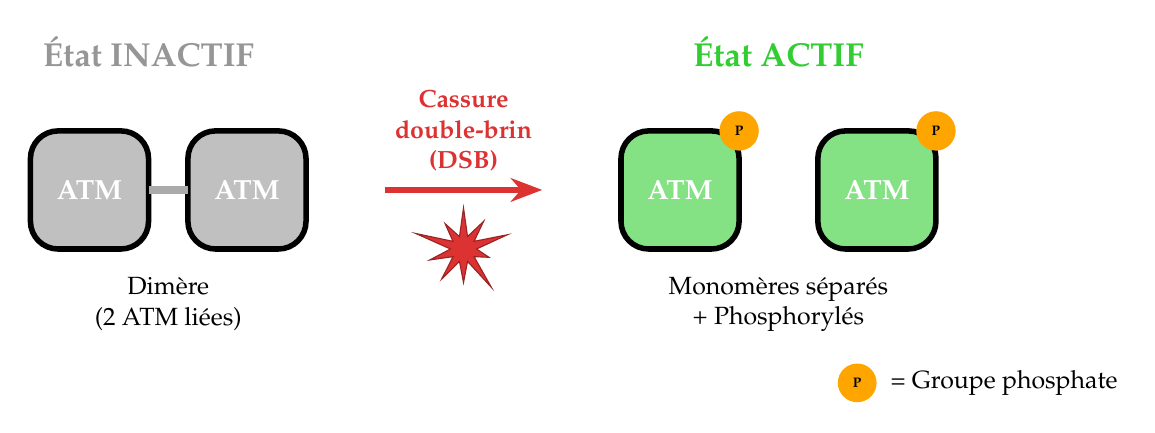
\begin{tikzpicture}[scale=1, transform shape]
    
    % === FORME INACTIVE (DIMÈRE) ===
    \node[font=\large\bfseries, color=atminactive] at (-4, 3) {État INACTIF};
    
    % Deux ATM liées (dimère)
    \draw[fill=atminactive!60, rounded corners=10pt, line width=2pt] (-5.5, 0.5) rectangle (-4, 2);
    \node[font=\bfseries, white] at (-4.75, 1.25) {ATM};
    
    \draw[fill=atminactive!60, rounded corners=10pt, line width=2pt] (-3.5, 0.5) rectangle (-2, 2);
    \node[font=\bfseries, white] at (-2.75, 1.25) {ATM};
    
    % Liaison entre les deux
    \draw[line width=3pt, atminactive!80] (-4, 1.25) -- (-3.5, 1.25);
    
    % Label dimère
    \node[font=\small, align=center] at (-3.75, -0.2) {Dimère\\(2 ATM liées)};
    
    % === FLÈCHE DE TRANSITION ===
    \draw[-{Stealth[length=4mm, width=3mm]}, line width=2pt, dsbcolor] (-1, 1.25) -- (1, 1.25);
    \node[font=\small\bfseries, dsbcolor, align=center] at (0, 2) {Cassure\\double-brin\\(DSB)};
    
    % Symbole DSB
    \node[starburst, starburst points=10, fill=dsbcolor, minimum size=0.8cm, draw=dsbcolor!70!black] at (0, 0.5) {};
    
    % === FORME ACTIVE (MONOMÈRES) ===
    \node[font=\large\bfseries, color=atmactive] at (4, 3) {État ACTIF};
    
    % Premier monomère avec phosphate
    \draw[fill=atmactive!60, rounded corners=10pt, line width=2pt] (2, 0.5) rectangle (3.5, 2);
    \node[font=\bfseries, white] at (2.75, 1.25) {ATM};
    \node[circle, fill=phosphocolor, minimum size=0.5cm, font=\tiny\bfseries] at (3.5, 2) {P};
    
    % Deuxième monomère avec phosphate
    \draw[fill=atmactive!60, rounded corners=10pt, line width=2pt] (4.5, 0.5) rectangle (6, 2);
    \node[font=\bfseries, white] at (5.25, 1.25) {ATM};
    \node[circle, fill=phosphocolor, minimum size=0.5cm, font=\tiny\bfseries] at (6, 2) {P};
    
    % Label monomères
    \node[font=\small, align=center] at (4, -0.2) {Monomères séparés\\+ Phosphorylés};
    
    % Légende phosphate
    \node[circle, fill=phosphocolor, minimum size=0.4cm, font=\tiny\bfseries] at (5, -1.2) {P};
    \node[font=\small, right] at (5.3, -1.2) {= Groupe phosphate};
    
\end{tikzpicture}
\caption{\textbf{Activation d'ATM par autophosphorylation.} À l'état normal, ATM existe sous forme de dimère inactif. La détection d'une cassure double-brin (DSB) provoque la séparation du dimère et l'autophosphorylation des monomères, les rendant actifs.}
\end{figure}

%==============================================================================
% FIGURE 2 : Mécanisme en 3 étapes
%==============================================================================
\section{Mécanisme d'activation en 3 étapes}

\begin{figure}[h!]
\centering
\begin{tikzpicture}[scale=0.9, transform shape,
    box/.style={rectangle, rounded corners=8pt, minimum width=3cm, minimum height=2cm, line width=1.5pt, align=center},
    arrow/.style={-{Stealth[length=3mm]}, line width=2pt}
]
    
    % === ÉTAPE 1 : État normal ===
    \node[box, fill=atminactive!30, draw=atminactive] (step1) at (0, 0) {
        \textbf{ATM}\\[3pt]
        \textbf{Dimère}\\[3pt]
        \small Inactif
    };
    \node[font=\bfseries, atminactive!80] at (0, 1.8) {ÉTAPE 1};
    \node[font=\small, align=center] at (0, -1.5) {Surveillance\\normale};
    
    % === FLÈCHE 1→2 ===
    \draw[arrow, dsbcolor] (1.8, 0) -- (3.2, 0);
    \node[font=\small, dsbcolor, align=center] at (2.5, 0.7) {DSB\\détectée};
    
    % === ÉTAPE 2 : Détection ===
    \node[box, fill=yellow!30, draw=yellow!70!black] (step2) at (5, 0) {
        \textbf{ATM}\\[3pt]
        \textbf{reconnaît}\\[3pt]
        \small la cassure
    };
    \node[font=\bfseries, yellow!70!black] at (5, 1.8) {ÉTAPE 2};
    \node[font=\small, align=center] at (5, -1.5) {Recrutement\\au site de cassure};
    
    % Symbole ADN cassé
    \draw[dnacolor, line width=3pt] (4.2, -0.3) -- (4.5, -0.3);
    \draw[dnacolor, line width=3pt] (5.5, -0.3) -- (5.8, -0.3);
    \node[font=\tiny, dsbcolor] at (5, -0.3) {✂};
    
    % === FLÈCHE 2→3 ===
    \draw[arrow, phosphocolor] (6.8, 0) -- (8.2, 0);
    \node[font=\small, phosphocolor, align=center] at (7.5, 0.7) {Auto-\\phospho.};
    
    % === ÉTAPE 3 : Activation ===
    \node[box, fill=atmactive!30, draw=atmactive] (step3) at (10, 0) {
        \textbf{ATM}\\[3pt]
        \textbf{Monomère}\\[3pt]
        \small Actif
    };
    \node[circle, fill=phosphocolor, minimum size=0.4cm, font=\tiny\bfseries] at (11.3, 0.8) {P};
    \node[font=\bfseries, atmactive] at (10, 1.8) {ÉTAPE 3};
    \node[font=\small, align=center] at (10, -1.5) {Cascade de\\signalisation};
    
    % === FLÈCHE VERS CASCADE ===
    \draw[arrow, atmactive] (10, -2.3) -- (10, -3.5);
    
    % === CASCADE ===
    \node[rectangle, rounded corners, fill=atmactive!20, draw=atmactive, line width=1pt, align=center, font=\small] at (10, -4.5) {
        Chk2 → Cdc25 → CDK1\\[2pt]
        \textbf{ARRÊT du cycle G2/M}
    };
    
\end{tikzpicture}
\caption{\textbf{Les 3 étapes de l'activation d'ATM.} (1) ATM surveille l'ADN sous forme inactive. (2) Détection et recrutement au site de cassure. (3) Autophosphorylation et activation de la cascade de signalisation menant à l'arrêt du cycle cellulaire.}
\end{figure}

%==============================================================================
% FIGURE 3 : Lien avec HRS
%==============================================================================
\section{Pourquoi ATM explique l'hyper-radiosensibilité (HRS)}

\begin{figure}[h!]
\centering
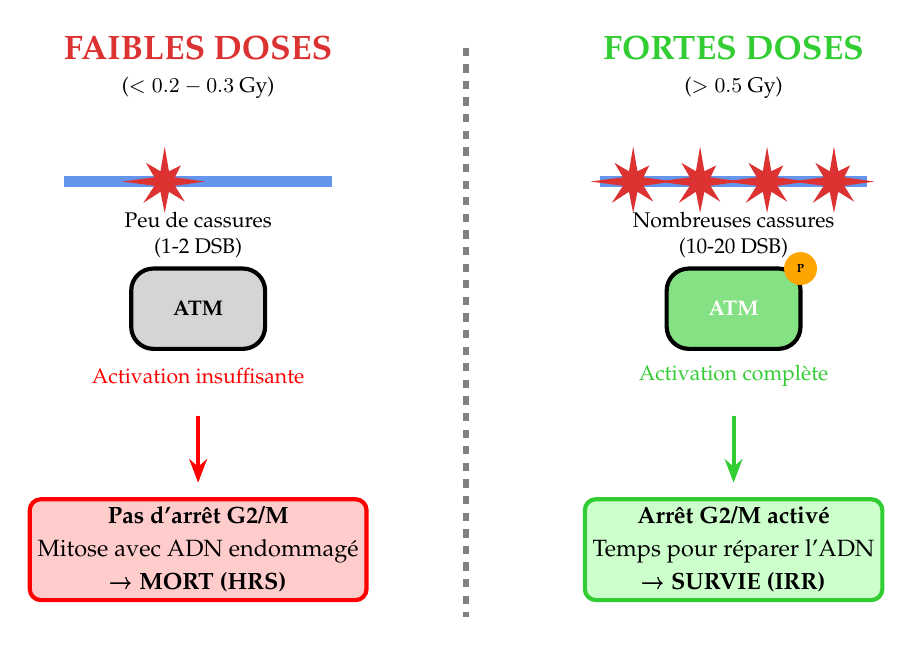
\begin{tikzpicture}[scale=0.85, transform shape]
    
    % === TITRE FAIBLES DOSES ===
    \node[font=\Large\bfseries, dsbcolor] at (-4, 4) {FAIBLES DOSES};
    \node[font=\small] at (-4, 3.4) {($< 0.2-0.3$ Gy)};
    
    % Peu de DSB
    \draw[dnacolor, line width=4pt] (-6, 2) -- (-2, 2);
    \node[starburst, starburst points=8, fill=dsbcolor, minimum size=0.3cm] at (-4.5, 2) {};
    \node[font=\small, align=center] at (-4, 1.2) {Peu de cassures\\(1-2 DSB)};
    
    % ATM pas assez activée
    \draw[fill=atminactive!40, rounded corners=8pt, line width=1.5pt] (-5, -0.5) rectangle (-3, 0.7);
    \node[font=\small\bfseries] at (-4, 0.1) {ATM};
    \node[font=\small, red] at (-4, -0.9) {Activation insuffisante};
    
    % Flèche vers conséquence
    \draw[-{Stealth[length=3mm]}, line width=1.5pt, red] (-4, -1.5) -- (-4, -2.5);
    
    % Conséquence
    \node[rectangle, rounded corners, fill=red!20, draw=red, line width=1.5pt, align=center] at (-4, -3.5) {
        \textbf{Pas d'arrêt G2/M}\\[2pt]
        Mitose avec ADN endommagé\\[2pt]
        \textbf{→ MORT (HRS)}
    };
    
    % === SÉPARATEUR ===
    \draw[line width=2pt, gray, dashed] (0, 4) -- (0, -4.5);
    
    % === TITRE FORTES DOSES ===
    \node[font=\Large\bfseries, atmactive] at (4, 4) {FORTES DOSES};
    \node[font=\small] at (4, 3.4) {($> 0.5$ Gy)};
    
    % Beaucoup de DSB
    \draw[dnacolor, line width=4pt] (2, 2) -- (6, 2);
    \node[starburst, starburst points=8, fill=dsbcolor, minimum size=0.3cm] at (2.5, 2) {};
    \node[starburst, starburst points=8, fill=dsbcolor, minimum size=0.3cm] at (3.5, 2) {};
    \node[starburst, starburst points=8, fill=dsbcolor, minimum size=0.3cm] at (4.5, 2) {};
    \node[starburst, starburst points=8, fill=dsbcolor, minimum size=0.3cm] at (5.5, 2) {};
    \node[font=\small, align=center] at (4, 1.2) {Nombreuses cassures\\(10-20 DSB)};
    
    % ATM bien activée
    \draw[fill=atmactive!60, rounded corners=8pt, line width=1.5pt] (3, -0.5) rectangle (5, 0.7);
    \node[font=\small\bfseries, white] at (4, 0.1) {ATM};
    \node[circle, fill=phosphocolor, minimum size=0.35cm, font=\tiny\bfseries] at (5, 0.7) {P};
    \node[font=\small, atmactive] at (4, -0.9) {Activation complète};
    
    % Flèche vers conséquence
    \draw[-{Stealth[length=3mm]}, line width=1.5pt, atmactive] (4, -1.5) -- (4, -2.5);
    
    % Conséquence
    \node[rectangle, rounded corners, fill=green!20, draw=atmactive, line width=1.5pt, align=center] at (4, -3.5) {
        \textbf{Arrêt G2/M activé}\\[2pt]
        Temps pour réparer l'ADN\\[2pt]
        \textbf{→ SURVIE (IRR)}
    };
    
\end{tikzpicture}
\caption{\textbf{ATM et le phénomène HRS/IRR.} À faibles doses, le nombre insuffisant de DSB ne permet pas d'activer pleinement ATM, entraînant une entrée en mitose avec de l'ADN endommagé (HRS). À fortes doses, ATM est pleinement activée, permettant l'arrêt du cycle et la réparation (IRR).}
\end{figure}

%==============================================================================
% RÉSUMÉ
%==============================================================================
\section{Résumé}

\begin{tcolorbox}[colback=atmcolor!10, colframe=atmcolor, title=\textbf{Points clés à retenir}]
\begin{enumerate}
    \item \textbf{ATM = Détecteur} : Protéine qui surveille l'intégrité de l'ADN
    \item \textbf{Autophosphorylation} : ATM s'active en ajoutant un phosphate sur elle-même
    \item \textbf{Dimère → Monomère} : La détection de DSB transforme ATM inactive en forme active
    \item \textbf{Seuil d'activation} : ATM nécessite un nombre minimum de DSB pour s'activer pleinement
    \item \textbf{Lien avec HRS} : Aux faibles doses, ATM insuffisamment activée → pas d'arrêt du cycle → mort cellulaire accrue
\end{enumerate}
\end{tcolorbox}

\vspace{0.5cm}

\begin{center}
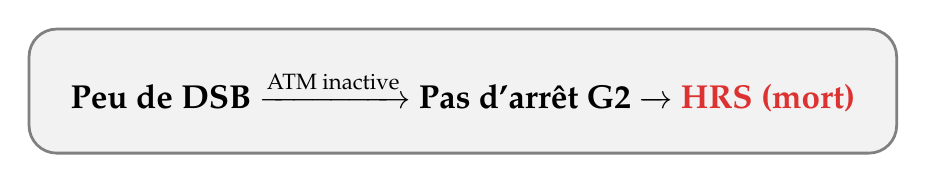
\begin{tikzpicture}
    % Équation résumé
    \node[rectangle, rounded corners=10pt, fill=gray!10, draw=gray, line width=1pt, inner sep=15pt, font=\large] {
        \textbf{Peu de DSB} $\xrightarrow{\text{ATM inactive}}$ \textbf{Pas d'arrêt G2} $\xrightarrow{}$ \textcolor{dsbcolor}{\textbf{HRS (mort)}}
    };
\end{tikzpicture}

\vspace{0.3cm}

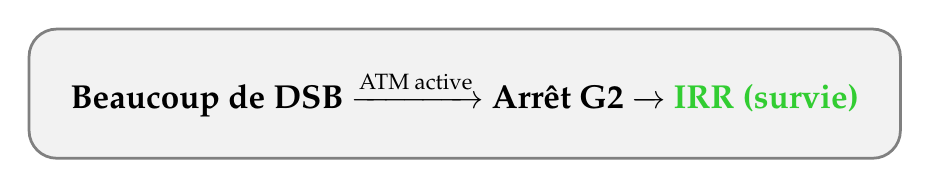
\begin{tikzpicture}
    \node[rectangle, rounded corners=10pt, fill=gray!10, draw=gray, line width=1pt, inner sep=15pt, font=\large] {
        \textbf{Beaucoup de DSB} $\xrightarrow{\text{ATM active}}$ \textbf{Arrêt G2} $\xrightarrow{}$ \textcolor{atmactive}{\textbf{IRR (survie)}}
    };
\end{tikzpicture}
\end{center}

\end{document}
